\section{Determining distance traveled from velocity} \label{S:4.1.VelocityDistance}

\vspace*{-14 pt}
\{\% include motivating-quest-top.md \%\}
\begin{itemize}
\item If we know the velocity of a moving body at every point in a given interval, can we determine the distance the object has traveled on the time interval?
\item How is the problem of finding distance traveled related to finding the area under a certain curve?
\item What does it mean to antidifferentiate a function and why is this process relevant to finding distance traveled?
\item If velocity is negative, how does this impact the problem of finding distance traveled?
\end{itemize}
\{\% include motivating-quest-bot.md \%\}

\subsection*{Introduction}

In the very first section of the text, we considered a situation where a moving object had a known position at time $t$.  In particular, we stipulated that a tennis ball tossed into the air had its height $s$ (in feet) at time $t$ (in seconds) given by $s(t) = 64 - 16(t-1)^2$.  From this starting point, we investigated the average velocity of the ball on a given interval $[a,b]$, computed by the difference quotient $\frac{s(b)-s(a)}{b-a}$, and eventually found that we could determine the exact instantaneous velocity of the ball at time $t$ by taking the derivative of the position function,
$$s'(t) = \lim_{h \to 0} \frac{s(t+h)-s(t)}{h}.$$
Thus, given a differentiable position function, we are able to know the exact velocity of the moving object at any point in time.

Moreover, from this foundational problem involving position and velocity we have learned a great deal.  Given a differentiable function $f$, we are now able to find its derivative and use this derivative to determine the function's instantaneous rate of change at any point in the domain, as well as to find where the function is increasing or decreasing, is concave up or concave down, and has relative extremes.  The vast majority of the problems and applications we have considered have involved the situation where a particular function is known and we seek information that relies on knowing the function's instantaneous rate of change.  That is, we have typically proceeded from a function $f$ to its derivative, $f'$, and then used the meaning of the derivative to help us answer important questions.  

In a much smaller number of situations so far, we have encountered the reverse situation where we instead know the derivative, $f'$, and have tried to deduce information about $f$.  It is this particular problem that will be the focus of our attention in most of Chapter~\ref{C:4}: if we know the instantaneous rate of change of a function, are we able to determine the function itself?  To begin, we start with a more focused question:  if we know the instantaneous velocity of an object moving along a straight line path, can we determine its corresponding position function? 

\{\% include previews/4.1.PA1.md \%\}

\subsection*{Area under the graph of the velocity function}\index{area!under velocity function}

In Preview Activity~\ref{PA:4.1}, we encountered a fundamental fact:  when a moving object's velocity is constant (and positive), the area under the velocity curve over a given interval tells us the distance the object traveled.   
\begin{figure}[h]
\begin{center}
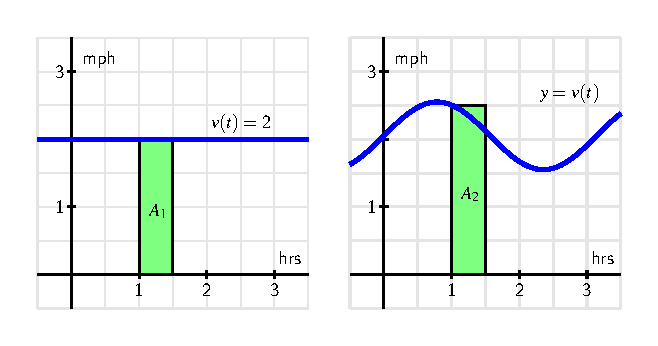
\includegraphics{figures/4_1_VelArea.eps}
\caption{At left, a constant velocity function; at right, a non-constant velocity function.} \label{F:4.1.VelArea}
\end{center}
\end{figure}
As seen at left in Figure~\ref{F:4.1.VelArea}, if we consider an object moving at 2 miles per hour over the time interval $[1,1.5]$, then the area $A_1$ of the shaded region under $y = v(t)$ on $[1,1.5]$ is
$$A _1= 2 \, \frac{\mbox{miles}}{\mbox{hour}} \cdot \frac{1}{2} \, \mbox{hours} = 1 \, \mbox{mile}.$$
This principle holds in general simply due to the fact that distance equals rate times time, provided the rate is constant.  Thus, if $v(t)$ is constant on the interval $[a,b]$, then the distance traveled on $[a,b]$ is the area $A$ that is given by 
$$A = v(a) (b-a) = v(a) \triangle t,$$
where $\triangle t$ is the change in $t$ over the interval.  Note, too, that we could use any value of $v(t)$ on the interval $[a,b]$, since the velocity is constant; we simply chose $v(a)$, the value at the interval's left endpoint.  For several examples where the velocity function is piecewise constant, see \href{http://gvsu.edu/s/9T}{\texttt{http://gvsu.edu/s/9T}}.\footnote{Marc Renault, calculus applets.}	

The situation is obviously more complicated when the velocity function is not constant.  At the same time, on relatively small intervals on which $v(t)$ does not vary much, the area principle allows us to estimate the distance the moving object travels on that time interval.  For instance, for the non-constant velocity function shown at right in Figure~\ref{F:4.1.VelArea}, we see that on the interval $[1,1.5]$, velocity varies from $v(1) = 2.5$ down to $v(1.5) \approx 2.1$.  Hence, one estimate for distance traveled is the area of the pictured rectangle, 
$$A_2 = v(1) \triangle t = 2.5 \, \frac{\mbox{miles}}{\mbox{hour}} \cdot \frac{1}{2} \, \mbox{hours} = 1.25 \, \mbox{miles}.$$
Because $v$ is decreasing on $[1,1.5]$ and the rectangle lies above the curve, clearly $A_2 = 1.25$ is an over-estimate of the actual distance traveled.

If we want to estimate the area under the non-constant velocity function on a wider interval, say $[0,3]$, it becomes apparent that one rectangle probably will not give a good approximation.  Instead, we could use the six rectangles pictured in Figure~\ref{F:4.1.VelArea2},  
\begin{figure}[h]
\begin{center}
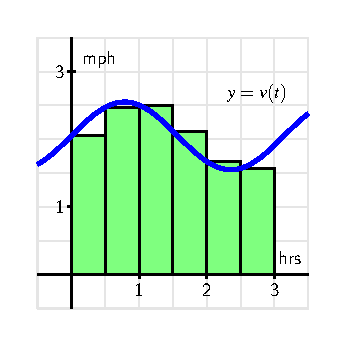
\includegraphics{figures/4_1_VelArea2.eps}
\caption{Using six rectangles to estimate the area under $y = v(t)$ on $[0,3]$.} \label{F:4.1.VelArea2}
\end{center}
\end{figure}
find the area of each rectangle, and add up the total.  Obviously there are choices to make and issues to understand: how many rectangles should we use?  where should we evaluate the function to decide the rectangle's height?  what happens if velocity is sometimes negative?  can we attain the exact area under any non-constant curve?  These questions and more are ones we will study in what follows; for now it suffices to realize that the simple idea of the area of a rectangle gives us a powerful tool for estimating both distance traveled from a velocity function as well as the area under an arbitrary curve.  To explore the setting of multiple rectangles to approximate area under a non-constant velocity function, see the applet found at \href{http://gvsu.edu/s/9U}{\texttt{http://gvsu.edu/s/9U}}.\footnote{Marc Renault, calculus applets.}

\{\% include activities/4.1.Act1.md \%\}

\subsection*{Two approaches: area and antidifferentiation}\index{antidifferentiation}\index{distance traveled}

When the velocity of a moving object is positive, the object's position is always increasing.  While we will soon consider situations where velocity is negative and think about the ramifications of this condition on distance traveled, for now we continue to assume that we are working with a positive velocity function.  In that setting, we have established that whenever $v$ is actually constant, the exact distance traveled on an interval is the area under the velocity curve; furthermore, we have observed that when $v$ is not constant, we can estimate the total distance traveled by finding the areas of rectangles that help to approximate the area under the velocity curve on the given interval.  Hence, we see the importance of the problem of finding the area between a curve and the horizontal axis:  besides being an interesting geometric question, in the setting of the curve being the (positive) velocity of a moving object, the area under the curve over an interval tells us the exact distance traveled on the interval.  We can estimate this area any time we have a graph of the velocity function or a table of data that tells us some relevant values of the function.

In Activity~\ref{A:4.1.1}, we also encountered an alternate approach to finding the distance traveled.  In particular, if we know a formula for the instantaneous velocity, $y = v(t)$, of the moving body at time $t$, then we realize that $v$ must be the derivative of some corresponding position function $s$.  If we can find a formula for $s$ from the formula for $v$, it follows that we know the position of the object at time $t$.  In addition, under the assumption that velocity is positive, the change in position over a given interval then tells us the distance traveled on that interval.  

For a simple example, consider the situation from Preview Activity~\ref{PA:4.1}, where a person is walking along a straight line and has velocity function $v(t) = 3$ mph.
\begin{figure}[h]
\begin{center}
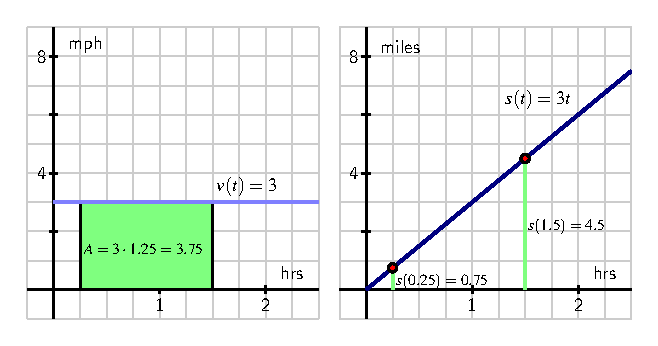
\includegraphics{figures/4_1_PA1Soln.eps}
\caption{The velocity function $v(t) = 3$ and corresponding position function $s(t) = 3t$.} \label{F:4.1.PA1Soln}
\end{center}
\end{figure}
As pictured in Figure~\ref{F:4.1.PA1Soln}, we see the already noted relationship between area and distance traveled on the left-hand graph of the velocity function.  In addition, because the velocity is constant at 3, we know that if\footnote{Here we are making the implicit assumption that $s(0) = 0$; we will further discuss the different possibilities for values of $s(0)$ in subsequent study.} $s(t) = 3t$, then $s'(t) = 3$, so $s(t) = 3t$ is a function whose derivative is $v(t)$.  Furthermore, we now observe that $s(1.5) = 4.5$ and $s(0.25) = 0.75$, which are the respective locations of the person at times $t = 0.25$ and $t = 1.5$, and therefore
$$s(1.5) - s(0.25) = 4.5 - 0.75 = 3.75 \ \mbox{miles}.$$
This is not only the change in position on $[0.25,1.5]$, but also precisely the distance traveled on $[0.25,1.5]$, which can also be computed by finding the area under the velocity curve over the same interval.  There are profound ideas and connections present in this example that we will spend much of the remainder of Chapter~\ref{C:4} studying and exploring.

For now, it is most important to observe that if we are given a formula for a velocity function $v$, it can be very helpful to find a function $s$ that satisfies $s' = v$.  In this context, we say that $s$ is an \emph{antiderivative} of $v$.  More generally, just as we say that $f'$ is the derivative of $f$ for a given function $f$, if we are given a function $g$ and $G$ is a function such that $G' = g$, we say that $G$ is an \emph{antiderivative} \index{antiderivative} of $g$.  For example, if $g(x) = 3x^2 + 2x$, an antiderivative of $g$ is $G(x) = x^3 + x^2$, since $G'(x) = g(x)$.  Note that we say ``an'' antiderivative of $g$ rather than ``the'' antiderivative of $g$ because $H(x) = x^3 + x^2 + 5$ is also a function whose derivative is $g$, and thus $H$ is another antiderivative of $g$.  

\{\% include activities/4.1.Act2.md \%\}

\subsection*{When velocity is negative}

Most of our work in this section has occurred under the assumption that velocity is positive.  This hypothesis guarantees that the movement of the object under consideration is always in a single direction, and hence ensures that the moving body's change in position is the same as the distance it travels on a given interval.  As we saw in Activity~\ref{A:4.1.2}, there are natural settings in which a moving object's velocity is negative; we would like to understand this scenario fully as well.

Consider a simple example where a person goes for a walk on a beach along a stretch of very straight shoreline that runs east-west.  We can naturally assume that their initial position is $s(0) = 0$, and further stipulate that their position function increases as they move east from their starting location.  For instance, a position of $s = 1$ mile represents being one mile east of the start location, while $s = -1$ tells us the person is one mile west of where they began walking on the beach.  Now suppose the person walks in the following manner.  From the outset at $t = 0$, the person walks due east at a constant rate of $3$ mph for 1.5 hours.  After 1.5 hours, the person stops abruptly and begins walking due west at the constant rate of $4$ mph and does so for 0.5 hours.  Then, after another abrupt stop and start, the person resumes walking at a constant rate of $3$ mph to the east for one more hour.  What is the total distance the person traveled on the time interval $t = 0$ to $t = 3$?  What is the person's total change in position over that time?

On one hand, these are elementary questions to answer because the velocity involved is constant on each interval.  From $t = 0$ to $t = 1.5$, the person traveled $$D_{[0,1.5]} = 3 \ \mbox{miles per hour} \cdot 1.5 \ \mbox{hours} = 4.5 \ \mbox{miles}.$$  Similarly, on $t = 1.5$ to $t = 2$, having a different rate, the distance traveled is
$$D_{[1.5,2]} = 4 \ \mbox{miles per hour} \cdot 0.5 \ \mbox{hours} = 2 \ \mbox{miles}.$$
Finally, similar calculations reveal that in the final hour, the person walked
$$D_{[2,3]} = 3 \ \mbox{miles per hour} \cdot 1 \ \mbox{hours} = 3 \ \mbox{miles},$$
so the total distance traveled is
$$D = D_{[0,1.5]} + D_{[1.5,2]} + D_{[2,3]} = 4.5 + 2 + 3 = 9.5 \ \mbox{miles}.$$
Since the velocity on $1.5 < t < 2$ is actually $v = -4$, being negative to indication motion in the westward direction, this tells us that the person first walked 4.5 miles east, then 2 miles west, followed by 3 more miles east.  Thus, the walker's total change in position is
$$\mbox{change in position} = 4.5 - 2 + 3 = 5.5 \ \mbox{miles}.$$

While we have been able to answer these questions fairly easily, it is also important to think about this problem graphically in order that we can generalize our solution to the more complicated setting when velocity is not constant, as well as to note the particular impact that negative velocity has.
\begin{figure}[h]
\begin{center}
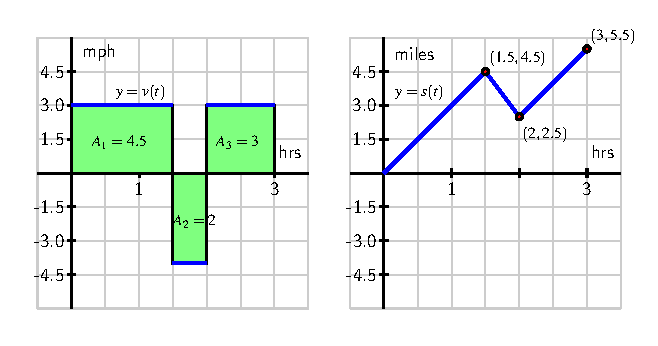
\includegraphics{figures/4_1_NegVel.eps}
\caption{At left, the velocity function of the person walking; at right, the corresponding position function.} \label{F:4.1.NegVel}
\end{center}
\end{figure}
In Figure~\ref{F:4.1.NegVel}, we see how the distances we computed above can be viewed as areas:  $A_1 = 4.5$ comes from taking rate times time ($3 \cdot 1.5$), as do $A_2$ and $A_3$ for the second and third rectangles.  The big new issue is that while $A_2$ is an area (and is therefore positive), because this area involves an interval on which the velocity function is negative, its area has a negative sign associated with it.  This helps us to distinguish between distance traveled and change in position.

The distance traveled is the sum of the areas, $$D = A_1 + A_2 + A_3 = 4.5 + 2 + 3 = 9.5 \ \mbox{miles}.$$ But the change in position has to account for the sign associated with the area, where those above the $t$-axis are considered positive while those below the $t$-axis are viewed as negative, so that 
$$s(3) - s(0) = (+4.5) + (-2) + (+3) = 5.5 \ \mbox{miles},$$
assigning the ``$-2$'' to the area in the interval $[1.5,2]$ because there velocity is negative and the person is walking in the ``negative'' direction.  In other words, the person walks 4.5 miles in the positive direction, followed by two miles in the negative direction, and then 3 more miles in the positive direction.  This affect of velocity being negative is also seen in the graph of the function $y=s(t)$, which has a negative slope (specifically, its slope is $-4$) on the interval $1.5<t<2$ since the velocity is $-4$ on that interval, which shows the person's position function is decreasing due to the fact that she is walking east, rather than west.  On the intervals where she is walking west, the velocity function is positive and the slope of the position function $s$ is therefore also positive.

To summarize, we see that if velocity is sometimes negative, this makes the moving object's change in position different from its distance traveled.  By viewing the intervals on which velocity is positive and negative separately, we may compute the distance traveled on each such interval, and then depending on whether we desire total distance traveled or total change in position, we may account for negative velocities that account for negative change in position, while still contributing positively to total distance traveled.  We close this section with one additional activity that further explores the effects of negative velocity on the problem of finding change in position and total distance traveled.

\{\% include activities/4.1.Act3.md \%\}


\{\% include motivating-quest-top.md \%\}
%\parbox{6.25 in}{
\begin{summary}
\item If we know the velocity of a moving body at every point in a given interval and the velocity is positive throughout, we can estimate the object's distance traveled and in some circumstances determine this value exactly.
\item In particular, when velocity is positive on an interval, we can find the total distance traveled by finding the area under the velocity curve and above the $t$-axis on the given time interval.  We may only be able to estimate this area, depending on the shape of the velocity curve.
\item An antiderivative of a function $f$ is a new function $F$ whose derivative is $f$.  That is, $F$ is an antiderivative of $f$ provided that $F' = f$.  In the context of velocity and position, if we know a velocity function $v$, an antiderivative of $v$ is a position function $s$ that satisfies $s' = v$.  If $v$ is positive on a given interval, say $[a,b]$, then the change in position, $s(b) - s(a)$, measures the distance the moving object traveled on $[a,b]$.
\item In the setting where velocity is sometimes negative, this means that the object is sometimes traveling in the opposite direction (depending on whether velocity is positive or negative), and thus involves the object backtracking.  To determine distance traveled, we have to think about the problem separately on intervals where velocity is positive and negative and account for the change in position on each such interval.
\end{summary}
%} \hspace*{3 pt}}

\nin \hrulefill

\newpage

\{\% include exercises/4.1.VelocityDistance(Ex).md \%\}

\clearpage
